\documentclass[a4paper]{tufte-handout}

% ams
\usepackage{amssymb,amsmath}

\usepackage{ifxetex,ifluatex}
\usepackage{fixltx2e} % provides \textsubscript
\ifnum 0\ifxetex 1\fi\ifluatex 1\fi=0 % if pdftex
  \usepackage[T1]{fontenc}
  \usepackage[utf8]{inputenc}
\else % if luatex or xelatex
  \makeatletter
  \@ifpackageloaded{fontspec}{}{\usepackage{fontspec}}
  \makeatother
  \defaultfontfeatures{Ligatures=TeX,Scale=MatchLowercase}
  \makeatletter
  \@ifpackageloaded{soul}{
     \renewcommand\allcapsspacing[1]{{\addfontfeature{LetterSpace=15}#1}}
     \renewcommand\smallcapsspacing[1]{{\addfontfeature{LetterSpace=10}#1}}
   }{}
  \makeatother

\fi

% graphix
\usepackage{graphicx}
\setkeys{Gin}{width=\linewidth,totalheight=\textheight,keepaspectratio}

% booktabs
\usepackage{booktabs}

% url
\usepackage{url}

% hyperref
\usepackage{hyperref}

% units.
\usepackage{units}


\setcounter{secnumdepth}{-1}

% citations
\usepackage{natbib}
\bibliographystyle{plainnat}


% pandoc syntax highlighting
\usepackage{color}
\usepackage{fancyvrb}
\newcommand{\VerbBar}{|}
\newcommand{\VERB}{\Verb[commandchars=\\\{\}]}
\DefineVerbatimEnvironment{Highlighting}{Verbatim}{commandchars=\\\{\}}
% Add ',fontsize=\small' for more characters per line
\newenvironment{Shaded}{}{}
\newcommand{\AlertTok}[1]{\textcolor[rgb]{1.00,0.00,0.00}{\textbf{#1}}}
\newcommand{\AnnotationTok}[1]{\textcolor[rgb]{0.38,0.63,0.69}{\textbf{\textit{#1}}}}
\newcommand{\AttributeTok}[1]{\textcolor[rgb]{0.49,0.56,0.16}{#1}}
\newcommand{\BaseNTok}[1]{\textcolor[rgb]{0.25,0.63,0.44}{#1}}
\newcommand{\BuiltInTok}[1]{#1}
\newcommand{\CharTok}[1]{\textcolor[rgb]{0.25,0.44,0.63}{#1}}
\newcommand{\CommentTok}[1]{\textcolor[rgb]{0.38,0.63,0.69}{\textit{#1}}}
\newcommand{\CommentVarTok}[1]{\textcolor[rgb]{0.38,0.63,0.69}{\textbf{\textit{#1}}}}
\newcommand{\ConstantTok}[1]{\textcolor[rgb]{0.53,0.00,0.00}{#1}}
\newcommand{\ControlFlowTok}[1]{\textcolor[rgb]{0.00,0.44,0.13}{\textbf{#1}}}
\newcommand{\DataTypeTok}[1]{\textcolor[rgb]{0.56,0.13,0.00}{#1}}
\newcommand{\DecValTok}[1]{\textcolor[rgb]{0.25,0.63,0.44}{#1}}
\newcommand{\DocumentationTok}[1]{\textcolor[rgb]{0.73,0.13,0.13}{\textit{#1}}}
\newcommand{\ErrorTok}[1]{\textcolor[rgb]{1.00,0.00,0.00}{\textbf{#1}}}
\newcommand{\ExtensionTok}[1]{#1}
\newcommand{\FloatTok}[1]{\textcolor[rgb]{0.25,0.63,0.44}{#1}}
\newcommand{\FunctionTok}[1]{\textcolor[rgb]{0.02,0.16,0.49}{#1}}
\newcommand{\ImportTok}[1]{#1}
\newcommand{\InformationTok}[1]{\textcolor[rgb]{0.38,0.63,0.69}{\textbf{\textit{#1}}}}
\newcommand{\KeywordTok}[1]{\textcolor[rgb]{0.00,0.44,0.13}{\textbf{#1}}}
\newcommand{\NormalTok}[1]{#1}
\newcommand{\OperatorTok}[1]{\textcolor[rgb]{0.40,0.40,0.40}{#1}}
\newcommand{\OtherTok}[1]{\textcolor[rgb]{0.00,0.44,0.13}{#1}}
\newcommand{\PreprocessorTok}[1]{\textcolor[rgb]{0.74,0.48,0.00}{#1}}
\newcommand{\RegionMarkerTok}[1]{#1}
\newcommand{\SpecialCharTok}[1]{\textcolor[rgb]{0.25,0.44,0.63}{#1}}
\newcommand{\SpecialStringTok}[1]{\textcolor[rgb]{0.73,0.40,0.53}{#1}}
\newcommand{\StringTok}[1]{\textcolor[rgb]{0.25,0.44,0.63}{#1}}
\newcommand{\VariableTok}[1]{\textcolor[rgb]{0.10,0.09,0.49}{#1}}
\newcommand{\VerbatimStringTok}[1]{\textcolor[rgb]{0.25,0.44,0.63}{#1}}
\newcommand{\WarningTok}[1]{\textcolor[rgb]{0.38,0.63,0.69}{\textbf{\textit{#1}}}}

% longtable

% multiplecol
\usepackage{multicol}

% strikeout
\usepackage[normalem]{ulem}

% morefloats
\usepackage{morefloats}


% tightlist macro required by pandoc >= 1.14
\providecommand{\tightlist}{%
  \setlength{\itemsep}{0pt}\setlength{\parskip}{0pt}}

% title / author / date
\title[分散の加法性を視覚的に理解する(その4)]{分散の加法性を視覚的に理解する(その4)}
\author{Sampo Suzuki, CC 4.0 BY-NC-SA}
\date{2021-06-06}

% --- 参考資料 ----------------------------------------------------------------
% http://ctan.math.illinois.edu/language/japanese/zxjafont/zxjafont.pdf
% https://github.com/Gedevan-Aleksizde/Japan.R2019/blob/master/latex/preamble.tex
% https://teastat.blogspot.com/2019/01/bookdown.html

% --- Packages ----------------------------------------------------------------
% 日本語とtufte, kableExtraを使うために必要なTeXパッケージ指定
% \usepackage[pdfbox,tombo]{gentombow}    % トンボを設定する場合は有効にする
\usepackage{ifthen}                     % 条件分岐用 \ifthenelse{条件}{T}{F}
\usepackage{booktabs}                   % ここからkableExtra用パッケージ
\usepackage{longtable}                  % 
\usepackage{array}                      % 
\usepackage{multirow}                   % 
\usepackage{wrapfig}                    % 
\usepackage{float}                      % 
\usepackage{colortbl}                   % 
\usepackage{pdflscape}                  % 
\usepackage{tabu}                       % 
\usepackage{threeparttable}             % 
\usepackage{threeparttablex}            % 
\usepackage[normalem]{ulem}             % 
\usepackage{inputenc}                   % 
\usepackage{makecell}                   % 
\usepackage{xcolor}                     % ここまでkableExtra用
\usepackage{amsmath}                    % 
\usepackage{fontawesome5}               % fontawesomeを使うために必要
\usepackage{subfig}                     % 複数の図を並べる際に必要(古い?)
% \usepackage{subcaption}                 % 同上(新しい?)
\usepackage{zxjatype}                   % 日本語処理に必要
% \usepackage{xeCJK}                      % zxjatypeを読み込むと一緒に読み込まれる
\usepackage[noto]{zxjafont}             % Linux環境用
% \usepackage[haranoaji]{zxjafont}        % Windows環境用
% \usepackage[hiragino-pro]{zxjafont}     % macOS環境用(おそらく、駄目ならNotoで)
\usepackage{pxrubrica}                  % ルビ用
\usepackage{hyperref}                   % ハイパーリンク用必要?
% 以下のパッケージについては下記サイトを参照方
% http://www.yamamo10.jp/yamamoto/comp/latex/make_doc/box/box.php
% \usepackage{ascmac}                     % 別行で文書を囲む場合
% \usepackage{fancybox}                   % 行中で文書を囲む場合 fancybx ではない
% \usepackage{fancyhdr}                   % ヘッダー用

% https://ja.wikibooks.org/wiki/TeX/LaTeX%E5%85%A5%E9%96%80
% https://teastat.blogspot.com/2019/01/bookdown.html
\usepackage{booktabs}
\usepackage{longtable}
\usepackage{array}
\usepackage{multirow}
\usepackage{wrapfig}
\usepackage{float}
\usepackage{colortbl}
\usepackage{pdflscape}
\usepackage{tabu}
\usepackage{threeparttable}
\usepackage{threeparttablex}
\usepackage[normalem]{ulem}
\usepackage{makecell}
\usepackage{xcolor}

\begin{document}

\maketitle

\begin{abstract}
\noindent  正規分布とは異なる分布でも分散の加法性が成り立つことを確認します。
\end{abstract}



\hypertarget{tux5206ux5e03ux306eux5834ux5408}{%
\section{\texorpdfstring{\textbf{t分布の場合}}{t分布の場合}}\label{tux5206ux5e03ux306eux5834ux5408}}

 自由度\$df = \(と\)df = Inf\$のt分布の分散を以下の関数で計算します。

\begin{Shaded}
\begin{Highlighting}[numbers=left,,]
\NormalTok{ft }\OtherTok{\textless{}{-}} \ControlFlowTok{function}\NormalTok{(}\AttributeTok{i =} \ConstantTok{NA}\NormalTok{, }\AttributeTok{n =} \DecValTok{5000000}\NormalTok{) \{}
\NormalTok{  x }\OtherTok{\textless{}{-}} \FunctionTok{rt}\NormalTok{(}\AttributeTok{n =}\NormalTok{ n, }\AttributeTok{df =} \DecValTok{5}\NormalTok{)}
\NormalTok{  y }\OtherTok{\textless{}{-}} \FunctionTok{rt}\NormalTok{(}\AttributeTok{n =}\NormalTok{ n, }\AttributeTok{df =} \ConstantTok{Inf}\NormalTok{)}
\NormalTok{  df }\OtherTok{\textless{}{-}} \FunctionTok{data.frame}\NormalTok{(}\AttributeTok{no =}\NormalTok{ i,}
                   \AttributeTok{var.x =} \FunctionTok{var}\NormalTok{(x), }\AttributeTok{var.y =} \FunctionTok{var}\NormalTok{(y),}
                   \AttributeTok{var.xy =} \FunctionTok{var}\NormalTok{(x }\SpecialCharTok{+}\NormalTok{ y), }\AttributeTok{var.sum =} \FunctionTok{var}\NormalTok{(x) }\SpecialCharTok{+} \FunctionTok{var}\NormalTok{(y),}
                   \AttributeTok{cov2 =} \FunctionTok{cov}\NormalTok{(x, y) }\SpecialCharTok{*} \DecValTok{2}\NormalTok{)}
\NormalTok{  df }\OtherTok{\textless{}{-}} \FunctionTok{cor.test}\NormalTok{(x, y) }\SpecialCharTok{\%\textgreater{}\%}\NormalTok{ broom}\SpecialCharTok{::}\FunctionTok{tidy}\NormalTok{() }\SpecialCharTok{\%\textgreater{}\%}\NormalTok{ dplyr}\SpecialCharTok{::}\FunctionTok{bind\_cols}\NormalTok{(df)}
  \FunctionTok{return}\NormalTok{(df)}
\NormalTok{\}}
\end{Highlighting}
\end{Shaded}

\[\mbox{加法1:}var.xy = var(x + y), \mbox{加法2:}var.sum = var(x) + var(y)\]

\begin{figure}

{\centering \subfloat[$df = 5$\label{fig:unnamed-chunk-2-1}]{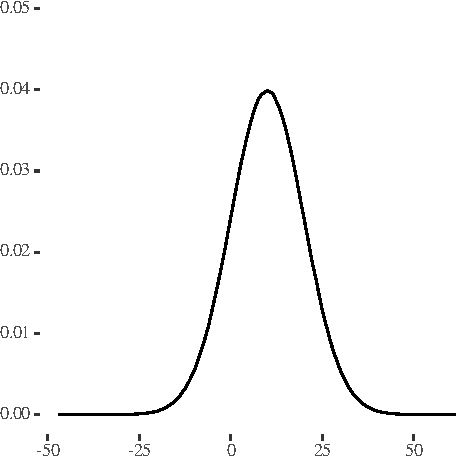
\includegraphics[width=0.4\linewidth]{AdditivityOfVariance4th_files/figure-latex/unnamed-chunk-2-1} }\subfloat[$df = \infty$\label{fig:unnamed-chunk-2-2}]{\includegraphics[width=0.4\linewidth]{AdditivityOfVariance4th_files/figure-latex/unnamed-chunk-2-2} }

}

\caption[分散を加算する二種類のt分布]{分散を加算する二種類のt分布}\label{fig:unnamed-chunk-2}
\end{figure}

\begin{table}

\caption{\label{tab:unnamed-chunk-4}計算結果}
\centering
\resizebox{\linewidth}{!}{
\begin{tabular}[t]{rrrrrrrrrr}
\toprule
No & 相関係数 & p値 & 標本x & 標本y & 加法1 & 加法2 & 差異 & 加法1/加法2 & cov2\\
\midrule
\cellcolor{gray!6}{1} & \cellcolor{gray!6}{-0.0003400} & \cellcolor{gray!6}{0.4471338} & \cellcolor{gray!6}{1.671315} & \cellcolor{gray!6}{1.0006527} & \cellcolor{gray!6}{2.671088} & \cellcolor{gray!6}{2.671968} & \cellcolor{gray!6}{-0.0008793} & \cellcolor{gray!6}{0.9996709} & \cellcolor{gray!6}{-0.0008793}\\
2 & -0.0001132 & 0.8001465 & 1.665842 & 1.0002102 & 2.665760 & 2.666052 & -0.0002923 & 0.9998904 & -0.0002923\\
\cellcolor{gray!6}{3} & \cellcolor{gray!6}{0.0001970} & \cellcolor{gray!6}{0.6595409} & \cellcolor{gray!6}{1.666911} & \cellcolor{gray!6}{1.0003627} & \cellcolor{gray!6}{2.667783} & \cellcolor{gray!6}{2.667274} & \cellcolor{gray!6}{0.0005088} & \cellcolor{gray!6}{1.0001908} & \cellcolor{gray!6}{0.0005088}\\
4 & 0.0002207 & 0.6216512 & 1.667868 & 1.0005398 & 2.668978 & 2.668408 & 0.0005702 & 1.0002137 & 0.0005702\\
\cellcolor{gray!6}{5} & \cellcolor{gray!6}{0.0003219} & \cellcolor{gray!6}{0.4716171} & \cellcolor{gray!6}{1.665999} & \cellcolor{gray!6}{1.0010391} & \cellcolor{gray!6}{2.667870} & \cellcolor{gray!6}{2.667038} & \cellcolor{gray!6}{0.0008315} & \cellcolor{gray!6}{1.0003118} & \cellcolor{gray!6}{0.0008315}\\
\addlinespace
6 & -0.0001162 & 0.7950144 & 1.668415 & 0.9996618 & 2.667776 & 2.668076 & -0.0003001 & 0.9998875 & -0.0003001\\
\cellcolor{gray!6}{7} & \cellcolor{gray!6}{0.0002744} & \cellcolor{gray!6}{0.5394774} & \cellcolor{gray!6}{1.667536} & \cellcolor{gray!6}{1.0018700} & \cellcolor{gray!6}{2.670115} & \cellcolor{gray!6}{2.669405} & \cellcolor{gray!6}{0.0007094} & \cellcolor{gray!6}{1.0002657} & \cellcolor{gray!6}{0.0007094}\\
8 & 0.0005338 & 0.2326176 & 1.665655 & 0.9998358 & 2.666869 & 2.665491 & 0.0013778 & 1.0005169 & 0.0013778\\
\cellcolor{gray!6}{9} & \cellcolor{gray!6}{0.0005526} & \cellcolor{gray!6}{0.2166069} & \cellcolor{gray!6}{1.668738} & \cellcolor{gray!6}{0.9999556} & \cellcolor{gray!6}{2.670121} & \cellcolor{gray!6}{2.668693} & \cellcolor{gray!6}{0.0014276} & \cellcolor{gray!6}{1.0005349} & \cellcolor{gray!6}{0.0014276}\\
10 & -0.0009500 & 0.0336438 & 1.670255 & 1.0000601 & 2.667859 & 2.670315 & -0.0024557 & 0.9990804 & -0.0024557\\
\addlinespace
\cellcolor{gray!6}{11} & \cellcolor{gray!6}{-0.0004474} & \cellcolor{gray!6}{0.3170860} & \cellcolor{gray!6}{1.668672} & \cellcolor{gray!6}{0.9997065} & \cellcolor{gray!6}{2.667223} & \cellcolor{gray!6}{2.668379} & \cellcolor{gray!6}{-0.0011558} & \cellcolor{gray!6}{0.9995669} & \cellcolor{gray!6}{-0.0011558}\\
12 & 0.0003121 & 0.4852412 & 1.669184 & 0.9993104 & 2.669301 & 2.668494 & 0.0008062 & 1.0003021 & 0.0008062\\
\cellcolor{gray!6}{13} & \cellcolor{gray!6}{-0.0007914} & \cellcolor{gray!6}{0.0767747} & \cellcolor{gray!6}{1.663218} & \cellcolor{gray!6}{1.0007921} & \cellcolor{gray!6}{2.661968} & \cellcolor{gray!6}{2.664010} & \cellcolor{gray!6}{-0.0020422} & \cellcolor{gray!6}{0.9992334} & \cellcolor{gray!6}{-0.0020422}\\
14 & 0.0001397 & 0.7547932 & 1.665388 & 1.0000734 & 2.665822 & 2.665461 & 0.0003605 & 1.0001353 & 0.0003605\\
\cellcolor{gray!6}{15} & \cellcolor{gray!6}{-0.0000405} & \cellcolor{gray!6}{0.9278549} & \cellcolor{gray!6}{1.668708} & \cellcolor{gray!6}{0.9992771} & \cellcolor{gray!6}{2.667881} & \cellcolor{gray!6}{2.667985} & \cellcolor{gray!6}{-0.0001046} & \cellcolor{gray!6}{0.9999608} & \cellcolor{gray!6}{-0.0001046}\\
\addlinespace
16 & -0.0005011 & 0.2625260 & 1.663565 & 1.0007718 & 2.663044 & 2.664337 & -0.0012931 & 0.9995147 & -0.0012931\\
\cellcolor{gray!6}{17} & \cellcolor{gray!6}{-0.0006516} & \cellcolor{gray!6}{0.1450992} & \cellcolor{gray!6}{1.665783} & \cellcolor{gray!6}{0.9992144} & \cellcolor{gray!6}{2.663316} & \cellcolor{gray!6}{2.664997} & \cellcolor{gray!6}{-0.0016814} & \cellcolor{gray!6}{0.9993691} & \cellcolor{gray!6}{-0.0016814}\\
18 & 0.0003550 & 0.4272851 & 1.670817 & 0.9996750 & 2.671410 & 2.670492 & 0.0009176 & 1.0003436 & 0.0009176\\
\cellcolor{gray!6}{19} & \cellcolor{gray!6}{0.0005604} & \cellcolor{gray!6}{0.2102049} & \cellcolor{gray!6}{1.667328} & \cellcolor{gray!6}{1.0008842} & \cellcolor{gray!6}{2.669660} & \cellcolor{gray!6}{2.668212} & \cellcolor{gray!6}{0.0014478} & \cellcolor{gray!6}{1.0005426} & \cellcolor{gray!6}{0.0014478}\\
20 & -0.0003488 & 0.4353974 & 1.664794 & 1.0002748 & 2.664169 & 2.665069 & -0.0009003 & 0.9996622 & -0.0009003\\
\bottomrule
\end{tabular}}
\end{table}

\newpage

\hypertarget{chi2ux5206ux5e03ux306eux5834ux5408}{%
\section{\texorpdfstring{\textbf{\(\chi^2\)分布の場合}}{\textbackslash chi\^{}2分布の場合}}\label{chi2ux5206ux5e03ux306eux5834ux5408}}

 自由度\(df = 1\)と\(df = 3\)の\(\chi^2\)分布の分散を以下の関数で計算します。

\begin{Shaded}
\begin{Highlighting}[numbers=left,,]
\NormalTok{fchisq }\OtherTok{\textless{}{-}} \ControlFlowTok{function}\NormalTok{(}\AttributeTok{i =} \ConstantTok{NA}\NormalTok{, }\AttributeTok{n =} \DecValTok{5000000}\NormalTok{) \{}
\NormalTok{  x }\OtherTok{\textless{}{-}} \FunctionTok{rchisq}\NormalTok{(}\AttributeTok{n =}\NormalTok{ n, }\AttributeTok{df =} \DecValTok{1}\NormalTok{)}
\NormalTok{  y }\OtherTok{\textless{}{-}} \FunctionTok{rchisq}\NormalTok{(}\AttributeTok{n =}\NormalTok{ n, }\AttributeTok{df =} \DecValTok{3}\NormalTok{)}
\NormalTok{  df }\OtherTok{\textless{}{-}} \FunctionTok{data.frame}\NormalTok{(}\AttributeTok{no =}\NormalTok{ i,}
                   \AttributeTok{var.x =} \FunctionTok{var}\NormalTok{(x), }\AttributeTok{var.y =} \FunctionTok{var}\NormalTok{(y),}
                   \AttributeTok{var.xy =} \FunctionTok{var}\NormalTok{(x }\SpecialCharTok{+}\NormalTok{ y), }\AttributeTok{var.sum =} \FunctionTok{var}\NormalTok{(x) }\SpecialCharTok{+} \FunctionTok{var}\NormalTok{(y),}
                   \AttributeTok{cov2 =} \FunctionTok{cov}\NormalTok{(x, y) }\SpecialCharTok{*} \DecValTok{2}\NormalTok{)}
\NormalTok{  df }\OtherTok{\textless{}{-}} \FunctionTok{cor.test}\NormalTok{(x, y) }\SpecialCharTok{\%\textgreater{}\%}\NormalTok{ broom}\SpecialCharTok{::}\FunctionTok{tidy}\NormalTok{() }\SpecialCharTok{\%\textgreater{}\%}\NormalTok{ dplyr}\SpecialCharTok{::}\FunctionTok{bind\_cols}\NormalTok{(df)}
  \FunctionTok{return}\NormalTok{(df)}
\NormalTok{\}}
\end{Highlighting}
\end{Shaded}

\[\mbox{加法1:}var.xy = var(x + y), \mbox{加法2:}var.sum = var(x) + var(y)\]

\begin{figure}

{\centering \subfloat[$df = 1$\label{fig:unnamed-chunk-7-1}]{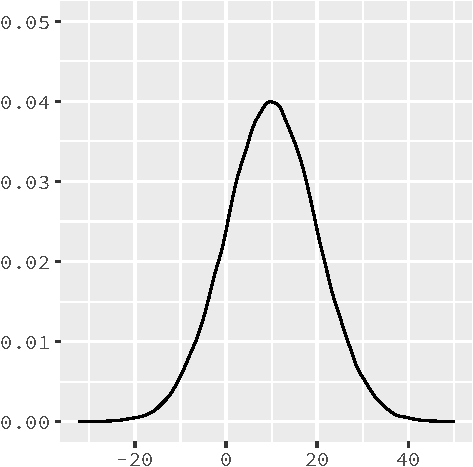
\includegraphics[width=0.4\linewidth]{AdditivityOfVariance4th_files/figure-latex/unnamed-chunk-7-1} }\subfloat[$df = 3$\label{fig:unnamed-chunk-7-2}]{\includegraphics[width=0.4\linewidth]{AdditivityOfVariance4th_files/figure-latex/unnamed-chunk-7-2} }

}

\caption[分散を加算する二種類の$\chi^2$分布]{分散を加算する二種類の$\chi^2$分布}\label{fig:unnamed-chunk-7}
\end{figure}

\begin{table}

\caption{\label{tab:unnamed-chunk-9}計算結果}
\centering
\resizebox{\linewidth}{!}{
\begin{tabular}[t]{rrrrrrrrrr}
\toprule
No & 相関係数 & p値 & 標本x & 標本y & 加法1 & 加法2 & 差異 & 加法1/加法2 & cov2\\
\midrule
\cellcolor{gray!6}{1} & \cellcolor{gray!6}{0.0004956} & \cellcolor{gray!6}{0.2677546} & \cellcolor{gray!6}{2.004440} & \cellcolor{gray!6}{6.012149} & \cellcolor{gray!6}{8.020031} & \cellcolor{gray!6}{8.016590} & \cellcolor{gray!6}{0.0034411} & \cellcolor{gray!6}{1.0004292} & \cellcolor{gray!6}{0.0034411}\\
2 & 0.0000173 & 0.9691781 & 1.997486 & 5.998751 & 7.996357 & 7.996237 & 0.0001196 & 1.0000150 & 0.0001196\\
\cellcolor{gray!6}{3} & \cellcolor{gray!6}{0.0000429} & \cellcolor{gray!6}{0.9236517} & \cellcolor{gray!6}{1.999706} & \cellcolor{gray!6}{6.012871} & \cellcolor{gray!6}{8.012874} & \cellcolor{gray!6}{8.012577} & \cellcolor{gray!6}{0.0002972} & \cellcolor{gray!6}{1.0000371} & \cellcolor{gray!6}{0.0002972}\\
4 & 0.0000098 & 0.9825511 & 1.997608 & 5.997723 & 7.995399 & 7.995331 & 0.0000677 & 1.0000085 & 0.0000677\\
\cellcolor{gray!6}{5} & \cellcolor{gray!6}{0.0003178} & \cellcolor{gray!6}{0.4772687} & \cellcolor{gray!6}{1.999837} & \cellcolor{gray!6}{5.988250} & \cellcolor{gray!6}{7.990287} & \cellcolor{gray!6}{7.988087} & \cellcolor{gray!6}{0.0021998} & \cellcolor{gray!6}{1.0002754} & \cellcolor{gray!6}{0.0021998}\\
\addlinespace
6 & -0.0007314 & 0.1019382 & 1.995278 & 5.993983 & 7.984202 & 7.989261 & -0.0050590 & 0.9993668 & -0.0050590\\
\cellcolor{gray!6}{7} & \cellcolor{gray!6}{-0.0002029} & \cellcolor{gray!6}{0.6500457} & \cellcolor{gray!6}{1.999653} & \cellcolor{gray!6}{5.996046} & \cellcolor{gray!6}{7.994294} & \cellcolor{gray!6}{7.995699} & \cellcolor{gray!6}{-0.0014051} & \cellcolor{gray!6}{0.9998243} & \cellcolor{gray!6}{-0.0014051}\\
8 & -0.0002943 & 0.5105458 & 1.998821 & 6.004295 & 8.001078 & 8.003117 & -0.0020388 & 0.9997452 & -0.0020388\\
\cellcolor{gray!6}{9} & \cellcolor{gray!6}{0.0000522} & \cellcolor{gray!6}{0.9070285} & \cellcolor{gray!6}{1.996728} & \cellcolor{gray!6}{5.992009} & \cellcolor{gray!6}{7.989099} & \cellcolor{gray!6}{7.988738} & \cellcolor{gray!6}{0.0003613} & \cellcolor{gray!6}{1.0000452} & \cellcolor{gray!6}{0.0003613}\\
10 & -0.0001619 & 0.7174116 & 1.997968 & 5.998410 & 7.995258 & 7.996379 & -0.0011207 & 0.9998599 & -0.0011207\\
\addlinespace
\cellcolor{gray!6}{11} & \cellcolor{gray!6}{0.0003936} & \cellcolor{gray!6}{0.3787565} & \cellcolor{gray!6}{1.998269} & \cellcolor{gray!6}{5.998312} & \cellcolor{gray!6}{7.999307} & \cellcolor{gray!6}{7.996581} & \cellcolor{gray!6}{0.0027256} & \cellcolor{gray!6}{1.0003408} & \cellcolor{gray!6}{0.0027256}\\
12 & 0.0001840 & 0.6807879 & 1.997278 & 5.997512 & 7.996063 & 7.994790 & 0.0012735 & 1.0001593 & 0.0012735\\
\cellcolor{gray!6}{13} & \cellcolor{gray!6}{-0.0003081} & \cellcolor{gray!6}{0.4909276} & \cellcolor{gray!6}{2.007474} & \cellcolor{gray!6}{6.003329} & \cellcolor{gray!6}{8.008665} & \cellcolor{gray!6}{8.010804} & \cellcolor{gray!6}{-0.0021389} & \cellcolor{gray!6}{0.9997330} & \cellcolor{gray!6}{-0.0021389}\\
14 & -0.0001352 & 0.7623968 & 2.006404 & 6.001392 & 8.006858 & 8.007796 & -0.0009384 & 0.9998828 & -0.0009384\\
\cellcolor{gray!6}{15} & \cellcolor{gray!6}{0.0000724} & \cellcolor{gray!6}{0.8714218} & \cellcolor{gray!6}{2.001221} & \cellcolor{gray!6}{5.999281} & \cellcolor{gray!6}{8.001004} & \cellcolor{gray!6}{8.000502} & \cellcolor{gray!6}{0.0005016} & \cellcolor{gray!6}{1.0000627} & \cellcolor{gray!6}{0.0005016}\\
\addlinespace
16 & -0.0005146 & 0.2498236 & 1.997352 & 6.002466 & 7.996254 & 7.999818 & -0.0035639 & 0.9995545 & -0.0035639\\
\cellcolor{gray!6}{17} & \cellcolor{gray!6}{0.0002133} & \cellcolor{gray!6}{0.6333729} & \cellcolor{gray!6}{1.997627} & \cellcolor{gray!6}{6.003839} & \cellcolor{gray!6}{8.002944} & \cellcolor{gray!6}{8.001467} & \cellcolor{gray!6}{0.0014775} & \cellcolor{gray!6}{1.0001847} & \cellcolor{gray!6}{0.0014775}\\
18 & -0.0004308 & 0.3354494 & 2.001473 & 6.002582 & 8.001068 & 8.004055 & -0.0029861 & 0.9996269 & -0.0029861\\
\cellcolor{gray!6}{19} & \cellcolor{gray!6}{0.0002259} & \cellcolor{gray!6}{0.6134288} & \cellcolor{gray!6}{1.995501} & \cellcolor{gray!6}{5.998105} & \cellcolor{gray!6}{7.995169} & \cellcolor{gray!6}{7.993606} & \cellcolor{gray!6}{0.0015633} & \cellcolor{gray!6}{1.0001956} & \cellcolor{gray!6}{0.0015633}\\
20 & -0.0006592 & 0.1404616 & 1.997356 & 6.002748 & 7.995539 & 8.000104 & -0.0045653 & 0.9994293 & -0.0045653\\
\bottomrule
\end{tabular}}
\end{table}

\newpage

\hypertarget{fux5206ux5e03ux306eux5834ux5408}{%
\section{\texorpdfstring{\textbf{F分布の場合}}{F分布の場合}}\label{fux5206ux5e03ux306eux5834ux5408}}

 自由度\(df_1 = 3, df_2 = 6\)と\(df_1 = 9, df_2 = 3\)のF分布の分散を以下の関数で計算します。

\begin{Shaded}
\begin{Highlighting}[numbers=left,,]
\NormalTok{ff }\OtherTok{\textless{}{-}} \ControlFlowTok{function}\NormalTok{(}\AttributeTok{i =} \ConstantTok{NA}\NormalTok{, }\AttributeTok{n =} \DecValTok{5000000}\NormalTok{) \{}
\NormalTok{  x }\OtherTok{\textless{}{-}} \FunctionTok{rf}\NormalTok{(}\AttributeTok{n =}\NormalTok{ n, }\AttributeTok{df1 =} \DecValTok{3}\NormalTok{, }\AttributeTok{df2 =} \DecValTok{6}\NormalTok{)}
\NormalTok{  y }\OtherTok{\textless{}{-}} \FunctionTok{rf}\NormalTok{(}\AttributeTok{n =}\NormalTok{ n, }\AttributeTok{df1 =} \DecValTok{9}\NormalTok{, }\AttributeTok{df2 =} \DecValTok{3}\NormalTok{)}
\NormalTok{  df }\OtherTok{\textless{}{-}} \FunctionTok{data.frame}\NormalTok{(}\AttributeTok{no =}\NormalTok{ i,}
                   \AttributeTok{var.x =} \FunctionTok{var}\NormalTok{(x), }\AttributeTok{var.y =} \FunctionTok{var}\NormalTok{(y),}
                   \AttributeTok{var.xy =} \FunctionTok{var}\NormalTok{(x }\SpecialCharTok{+}\NormalTok{ y), }\AttributeTok{var.sum =} \FunctionTok{var}\NormalTok{(x) }\SpecialCharTok{+} \FunctionTok{var}\NormalTok{(y),}
                   \AttributeTok{cov2 =} \FunctionTok{cov}\NormalTok{(x, y) }\SpecialCharTok{*} \DecValTok{2}\NormalTok{)}
\NormalTok{  df }\OtherTok{\textless{}{-}} \FunctionTok{cor.test}\NormalTok{(x, y) }\SpecialCharTok{\%\textgreater{}\%}\NormalTok{ broom}\SpecialCharTok{::}\FunctionTok{tidy}\NormalTok{() }\SpecialCharTok{\%\textgreater{}\%}\NormalTok{ dplyr}\SpecialCharTok{::}\FunctionTok{bind\_cols}\NormalTok{(df)}
  \FunctionTok{return}\NormalTok{(df)}
\NormalTok{\}}
\end{Highlighting}
\end{Shaded}

\[\mbox{加法1:}var.xy = var(x + y), \mbox{加法2:}var.sum = var(x) + var(y)\]

\begin{figure}

{\centering \subfloat[$df_1 = 3, df_2 =6$\label{fig:unnamed-chunk-11-1}]{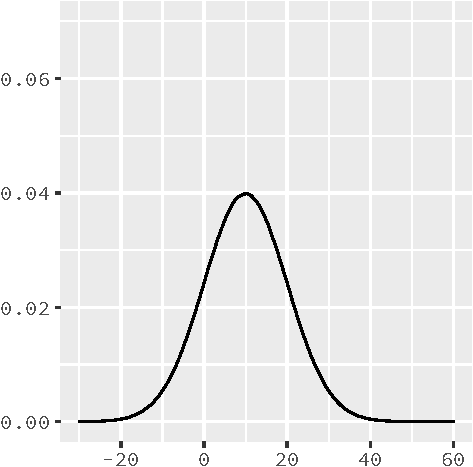
\includegraphics[width=0.4\linewidth]{AdditivityOfVariance4th_files/figure-latex/unnamed-chunk-11-1} }\subfloat[$df_1 = 9, df_2 = 3$\label{fig:unnamed-chunk-11-2}]{\includegraphics[width=0.4\linewidth]{AdditivityOfVariance4th_files/figure-latex/unnamed-chunk-11-2} }

}

\caption[分散を加算する二種類のF分布]{分散を加算する二種類のF分布}\label{fig:unnamed-chunk-11}
\end{figure}

\begin{table}

\caption{\label{tab:unnamed-chunk-13}計算結果}
\centering
\resizebox{\linewidth}{!}{
\begin{tabular}[t]{rrrrrrrrrr}
\toprule
No & 相関係数 & p値 & 標本x & 標本y & 加法1 & 加法2 & 差異 & 加法1/加法2 & cov2\\
\midrule
\cellcolor{gray!6}{1} & \cellcolor{gray!6}{-0.0005088} & \cellcolor{gray!6}{0.2552622} & \cellcolor{gray!6}{5.211667} & \cellcolor{gray!6}{2187.4152} & \cellcolor{gray!6}{2192.5182} & \cellcolor{gray!6}{2192.6269} & \cellcolor{gray!6}{-0.1086455} & \cellcolor{gray!6}{0.9999504} & \cellcolor{gray!6}{-0.1086455}\\
2 & -0.0000916 & 0.8376373 & 5.108454 & 1445.2154 & 1450.3081 & 1450.3239 & -0.0157483 & 0.9999891 & -0.0157483\\
\cellcolor{gray!6}{3} & \cellcolor{gray!6}{-0.0002445} & \cellcolor{gray!6}{0.5845768} & \cellcolor{gray!6}{5.199387} & \cellcolor{gray!6}{2018.1786} & \cellcolor{gray!6}{2023.3279} & \cellcolor{gray!6}{2023.3780} & \cellcolor{gray!6}{-0.0500910} & \cellcolor{gray!6}{0.9999752} & \cellcolor{gray!6}{-0.0500910}\\
4 & 0.0002644 & 0.5544113 & 5.122349 & 469.2528 & 474.4011 & 474.3752 & 0.0259233 & 1.0000546 & 0.0259233\\
\cellcolor{gray!6}{5} & \cellcolor{gray!6}{-0.0001986} & \cellcolor{gray!6}{0.6569190} & \cellcolor{gray!6}{5.215827} & \cellcolor{gray!6}{1280.2691} & \cellcolor{gray!6}{1285.4525} & \cellcolor{gray!6}{1285.4849} & \cellcolor{gray!6}{-0.0324644} & \cellcolor{gray!6}{0.9999747} & \cellcolor{gray!6}{-0.0324644}\\
\addlinespace
6 & -0.0002592 & 0.5622175 & 5.434277 & 1433.5962 & 1438.9847 & 1439.0304 & -0.0457532 & 0.9999682 & -0.0457532\\
\cellcolor{gray!6}{7} & \cellcolor{gray!6}{-0.0001976} & \cellcolor{gray!6}{0.6585898} & \cellcolor{gray!6}{5.176098} & \cellcolor{gray!6}{48599.2364} & \cellcolor{gray!6}{48604.2143} & \cellcolor{gray!6}{48604.4125} & \cellcolor{gray!6}{-0.1982197} & \cellcolor{gray!6}{0.9999959} & \cellcolor{gray!6}{-0.1982197}\\
8 & 0.0001127 & 0.8009720 & 5.074826 & 2330.8257 & 2335.9251 & 2335.9006 & 0.0245225 & 1.0000105 & 0.0245225\\
\cellcolor{gray!6}{9} & \cellcolor{gray!6}{-0.0002067} & \cellcolor{gray!6}{0.6439203} & \cellcolor{gray!6}{5.159144} & \cellcolor{gray!6}{1372.0367} & \cellcolor{gray!6}{1377.1611} & \cellcolor{gray!6}{1377.1959} & \cellcolor{gray!6}{-0.0347832} & \cellcolor{gray!6}{0.9999747} & \cellcolor{gray!6}{-0.0347832}\\
10 & -0.0003368 & 0.4514110 & 5.182321 & 744.9437 & 750.0842 & 750.1260 & -0.0418506 & 0.9999442 & -0.0418506\\
\addlinespace
\cellcolor{gray!6}{11} & \cellcolor{gray!6}{0.0001890} & \cellcolor{gray!6}{0.6725413} & \cellcolor{gray!6}{5.312891} & \cellcolor{gray!6}{748.5687} & \cellcolor{gray!6}{753.9055} & \cellcolor{gray!6}{753.8816} & \cellcolor{gray!6}{0.0238408} & \cellcolor{gray!6}{1.0000316} & \cellcolor{gray!6}{0.0238408}\\
12 & 0.0001013 & 0.8207210 & 5.098162 & 1298.4698 & 1303.5845 & 1303.5680 & 0.0164916 & 1.0000127 & 0.0164916\\
\cellcolor{gray!6}{13} & \cellcolor{gray!6}{0.0002387} & \cellcolor{gray!6}{0.5935867} & \cellcolor{gray!6}{5.178266} & \cellcolor{gray!6}{1903.9322} & \cellcolor{gray!6}{1909.1579} & \cellcolor{gray!6}{1909.1105} & \cellcolor{gray!6}{0.0473932} & \cellcolor{gray!6}{1.0000248} & \cellcolor{gray!6}{0.0473932}\\
14 & 0.0005441 & 0.2237773 & 5.220821 & 749.8635 & 755.1525 & 755.0844 & 0.0680822 & 1.0000902 & 0.0680822\\
\cellcolor{gray!6}{15} & \cellcolor{gray!6}{0.0002153} & \cellcolor{gray!6}{0.6302591} & \cellcolor{gray!6}{5.207314} & \cellcolor{gray!6}{1537.7464} & \cellcolor{gray!6}{1542.9922} & \cellcolor{gray!6}{1542.9537} & \cellcolor{gray!6}{0.0385271} & \cellcolor{gray!6}{1.0000250} & \cellcolor{gray!6}{0.0385271}\\
\addlinespace
16 & 0.0003802 & 0.3951848 & 5.181432 & 974.5329 & 979.7684 & 979.7144 & 0.0540401 & 1.0000552 & 0.0540401\\
\cellcolor{gray!6}{17} & \cellcolor{gray!6}{0.0003537} & \cellcolor{gray!6}{0.4289961} & \cellcolor{gray!6}{5.123908} & \cellcolor{gray!6}{648.6608} & \cellcolor{gray!6}{653.8255} & \cellcolor{gray!6}{653.7847} & \cellcolor{gray!6}{0.0407833} & \cellcolor{gray!6}{1.0000624} & \cellcolor{gray!6}{0.0407833}\\
18 & -0.0003690 & 0.4093272 & 5.272903 & 813.8613 & 819.0858 & 819.1342 & -0.0483437 & 0.9999410 & -0.0483437\\
\cellcolor{gray!6}{19} & \cellcolor{gray!6}{0.0002439} & \cellcolor{gray!6}{0.5854696} & \cellcolor{gray!6}{5.635600} & \cellcolor{gray!6}{933.4921} & \cellcolor{gray!6}{939.1631} & \cellcolor{gray!6}{939.1277} & \cellcolor{gray!6}{0.0353831} & \cellcolor{gray!6}{1.0000377} & \cellcolor{gray!6}{0.0353831}\\
20 & 0.0005904 & 0.1867975 & 5.529007 & 1510.8539 & 1516.4908 & 1516.3829 & 0.1079172 & 1.0000712 & 0.1079172\\
\bottomrule
\end{tabular}}
\end{table}

\newpage

\hypertarget{tux5206ux5e03ux3068chi2ux5206ux5e03ux306eux5834ux5408}{%
\section{\texorpdfstring{\textbf{t分布と\(\chi^2\)分布の場合}}{t分布と\textbackslash chi\^{}2分布の場合}}\label{tux5206ux5e03ux3068chi2ux5206ux5e03ux306eux5834ux5408}}

 自由度\(df = 5\)のt分布と\(df = 3\)の\(\chi^2\)分布の分散を以下の関数で計算します。

\begin{Shaded}
\begin{Highlighting}[numbers=left,,]
\NormalTok{ftchisq }\OtherTok{\textless{}{-}} \ControlFlowTok{function}\NormalTok{(}\AttributeTok{i =} \ConstantTok{NA}\NormalTok{, }\AttributeTok{n =} \DecValTok{5000000}\NormalTok{) \{}
\NormalTok{  x }\OtherTok{\textless{}{-}} \FunctionTok{rt}\NormalTok{(}\AttributeTok{n =}\NormalTok{ n, }\AttributeTok{df =} \DecValTok{5}\NormalTok{)}
\NormalTok{  y }\OtherTok{\textless{}{-}} \FunctionTok{rchisq}\NormalTok{(}\AttributeTok{n =}\NormalTok{ n, }\AttributeTok{df =} \DecValTok{3}\NormalTok{)}
\NormalTok{  df }\OtherTok{\textless{}{-}} \FunctionTok{data.frame}\NormalTok{(}\AttributeTok{no =}\NormalTok{ i,}
                   \AttributeTok{var.x =} \FunctionTok{var}\NormalTok{(x), }\AttributeTok{var.y =} \FunctionTok{var}\NormalTok{(y),}
                   \AttributeTok{var.xy =} \FunctionTok{var}\NormalTok{(x }\SpecialCharTok{+}\NormalTok{ y), }\AttributeTok{var.sum =} \FunctionTok{var}\NormalTok{(x) }\SpecialCharTok{+} \FunctionTok{var}\NormalTok{(y),}
                   \AttributeTok{cov2 =} \FunctionTok{cov}\NormalTok{(x, y) }\SpecialCharTok{*} \DecValTok{2}\NormalTok{)}
\NormalTok{  df }\OtherTok{\textless{}{-}} \FunctionTok{cor.test}\NormalTok{(x, y) }\SpecialCharTok{\%\textgreater{}\%}\NormalTok{ broom}\SpecialCharTok{::}\FunctionTok{tidy}\NormalTok{() }\SpecialCharTok{\%\textgreater{}\%}\NormalTok{ dplyr}\SpecialCharTok{::}\FunctionTok{bind\_cols}\NormalTok{(df)}
  \FunctionTok{return}\NormalTok{(df)}
\NormalTok{\}}
\end{Highlighting}
\end{Shaded}

\[\mbox{加法1:}var.xy = var(x + y), \mbox{加法2:}var.sum = var(x) + var(y)\]

\begin{figure}

{\centering \subfloat[$df = 5$\label{fig:unnamed-chunk-15-1}]{\includegraphics[width=0.4\linewidth]{AdditivityOfVariance4th_files/figure-latex/unnamed-chunk-15-1} }\subfloat[$df = 3$\label{fig:unnamed-chunk-15-2}]{\includegraphics[width=0.4\linewidth]{AdditivityOfVariance4th_files/figure-latex/unnamed-chunk-15-2} }

}

\caption[分散を加算する二種類の$\chi^2$分布]{分散を加算する二種類の$\chi^2$分布}\label{fig:unnamed-chunk-15}
\end{figure}

\begin{table}

\caption{\label{tab:unnamed-chunk-17}計算結果}
\centering
\resizebox{\linewidth}{!}{
\begin{tabular}[t]{rrrrrrrrrr}
\toprule
No & 相関係数 & p値 & 標本x & 標本y & 加法1 & 加法2 & 差異 & 加法1/加法2 & cov2\\
\midrule
\cellcolor{gray!6}{1} & \cellcolor{gray!6}{-0.0001782} & \cellcolor{gray!6}{0.6903304} & \cellcolor{gray!6}{1.664412} & \cellcolor{gray!6}{5.999207} & \cellcolor{gray!6}{7.662493} & \cellcolor{gray!6}{7.663619} & \cellcolor{gray!6}{-0.0011260} & \cellcolor{gray!6}{0.9998531} & \cellcolor{gray!6}{-0.0011260}\\
2 & -0.0002724 & 0.5425179 & 1.664679 & 6.004114 & 7.667071 & 7.668793 & -0.0017221 & 0.9997754 & -0.0017221\\
\cellcolor{gray!6}{3} & \cellcolor{gray!6}{-0.0001043} & \cellcolor{gray!6}{0.8155900} & \cellcolor{gray!6}{1.666044} & \cellcolor{gray!6}{5.991276} & \cellcolor{gray!6}{7.656660} & \cellcolor{gray!6}{7.657319} & \cellcolor{gray!6}{-0.0006590} & \cellcolor{gray!6}{0.9999139} & \cellcolor{gray!6}{-0.0006590}\\
4 & -0.0007060 & 0.1144232 & 1.666784 & 6.009416 & 7.671731 & 7.676200 & -0.0044687 & 0.9994179 & -0.0044687\\
\cellcolor{gray!6}{5} & \cellcolor{gray!6}{0.0005852} & \cellcolor{gray!6}{0.1906797} & \cellcolor{gray!6}{1.664959} & \cellcolor{gray!6}{5.998756} & \cellcolor{gray!6}{7.667414} & \cellcolor{gray!6}{7.663715} & \cellcolor{gray!6}{0.0036989} & \cellcolor{gray!6}{1.0004827} & \cellcolor{gray!6}{0.0036989}\\
\addlinespace
6 & -0.0008875 & 0.0472098 & 1.666058 & 5.995425 & 7.655873 & 7.661483 & -0.0056096 & 0.9992678 & -0.0056096\\
\cellcolor{gray!6}{7} & \cellcolor{gray!6}{0.0000842} & \cellcolor{gray!6}{0.8506780} & \cellcolor{gray!6}{1.667544} & \cellcolor{gray!6}{5.999345} & \cellcolor{gray!6}{7.667422} & \cellcolor{gray!6}{7.666890} & \cellcolor{gray!6}{0.0005326} & \cellcolor{gray!6}{1.0000695} & \cellcolor{gray!6}{0.0005326}\\
8 & 0.0001750 & 0.6955518 & 1.668354 & 6.008008 & 7.677471 & 7.676363 & 0.0011082 & 1.0001444 & 0.0011082\\
\cellcolor{gray!6}{9} & \cellcolor{gray!6}{-0.0000253} & \cellcolor{gray!6}{0.9549389} & \cellcolor{gray!6}{1.669423} & \cellcolor{gray!6}{6.001814} & \cellcolor{gray!6}{7.671077} & \cellcolor{gray!6}{7.671237} & \cellcolor{gray!6}{-0.0001600} & \cellcolor{gray!6}{0.9999791} & \cellcolor{gray!6}{-0.0001600}\\
10 & 0.0001198 & 0.7887721 & 1.668855 & 6.006666 & 7.676280 & 7.675521 & 0.0007587 & 1.0000988 & 0.0007587\\
\addlinespace
\cellcolor{gray!6}{11} & \cellcolor{gray!6}{0.0002645} & \cellcolor{gray!6}{0.5542274} & \cellcolor{gray!6}{1.668434} & \cellcolor{gray!6}{6.004580} & \cellcolor{gray!6}{7.674688} & \cellcolor{gray!6}{7.673014} & \cellcolor{gray!6}{0.0016744} & \cellcolor{gray!6}{1.0002182} & \cellcolor{gray!6}{0.0016744}\\
12 & -0.0003488 & 0.4354460 & 1.666775 & 5.999497 & 7.664066 & 7.666271 & -0.0022059 & 0.9997123 & -0.0022059\\
\cellcolor{gray!6}{13} & \cellcolor{gray!6}{0.0007602} & \cellcolor{gray!6}{0.0891628} & \cellcolor{gray!6}{1.663094} & \cellcolor{gray!6}{6.006085} & \cellcolor{gray!6}{7.673984} & \cellcolor{gray!6}{7.669179} & \cellcolor{gray!6}{0.0048051} & \cellcolor{gray!6}{1.0006266} & \cellcolor{gray!6}{0.0048051}\\
14 & -0.0000040 & 0.9928889 & 1.664894 & 5.995082 & 7.659951 & 7.659976 & -0.0000252 & 0.9999967 & -0.0000252\\
\cellcolor{gray!6}{15} & \cellcolor{gray!6}{0.0005534} & \cellcolor{gray!6}{0.2159302} & \cellcolor{gray!6}{1.669772} & \cellcolor{gray!6}{6.003873} & \cellcolor{gray!6}{7.677149} & \cellcolor{gray!6}{7.673645} & \cellcolor{gray!6}{0.0035043} & \cellcolor{gray!6}{1.0004567} & \cellcolor{gray!6}{0.0035043}\\
\addlinespace
16 & 0.0000438 & 0.9219608 & 1.666002 & 5.998464 & 7.664743 & 7.664466 & 0.0002770 & 1.0000361 & 0.0002770\\
\cellcolor{gray!6}{17} & \cellcolor{gray!6}{0.0002501} & \cellcolor{gray!6}{0.5760000} & \cellcolor{gray!6}{1.665924} & \cellcolor{gray!6}{6.003260} & \cellcolor{gray!6}{7.670766} & \cellcolor{gray!6}{7.669184} & \cellcolor{gray!6}{0.0015818} & \cellcolor{gray!6}{1.0002063} & \cellcolor{gray!6}{0.0015818}\\
18 & -0.0004545 & 0.3094799 & 1.665073 & 5.992650 & 7.654852 & 7.657724 & -0.0028714 & 0.9996250 & -0.0028714\\
\cellcolor{gray!6}{19} & \cellcolor{gray!6}{-0.0002343} & \cellcolor{gray!6}{0.6003523} & \cellcolor{gray!6}{1.664831} & \cellcolor{gray!6}{6.006462} & \cellcolor{gray!6}{7.669810} & \cellcolor{gray!6}{7.671292} & \cellcolor{gray!6}{-0.0014818} & \cellcolor{gray!6}{0.9998068} & \cellcolor{gray!6}{-0.0014818}\\
20 & 0.0001036 & 0.8167538 & 1.670891 & 6.008467 & 7.680015 & 7.679358 & 0.0006567 & 1.0000855 & 0.0006567\\
\bottomrule
\end{tabular}}
\end{table}

\bibliography{bib/references.bib}



\end{document}
